\documentclass{article}
\usepackage[utf8]{inputenc}
\usepackage[italian]{babel}
\usepackage[T1]{fontenc}
\usepackage{blindtext}
\usepackage{indentfirst}
\usepackage{array}
\usepackage{titlesec}
\usepackage{multicol}
\usepackage{graphicx}
\usepackage{float}
\usepackage{listings}
\usepackage{url}
\graphicspath{ {./Immagini/} }
\titleformat{\subsection}[runin]{\normalfont\bfseries}{\thesubsection}{0.5em}{}

% Margins
\addtolength{\textwidth}{1.0in}
\addtolength{\textheight}{2.0in}
\addtolength{\evensidemargin}{-0.75in}
\addtolength{\oddsidemargin}{-0.75in}
\addtolength{\topmargin}{-1.0in}

\begin{document}

% Title & author
\title{Esercizio 1}
\author{Giovanni Stefanini - 6182949}
\date{Aprile 2021}
\maketitle


\section{Introduzione}
In questo esercizio è stato prima implementato una funzione che generasse un vettore casuale, e in seguito sono stati implementati gli algoritmi di InsertionSort() e QuickSort(). Il tutto è stato implementato nel file {\em Es1ASD.py}.

In particolare nel file {\em Test1ASD.py} sono stati poi implementati delle funzioni che testassero gli algoritmi applicandoli ad array di dimensioni crescenti con valori casuali, e prendendo come elemento di riferimento per la qualità dell'algoritmo il {\em \bf tempo di esecuzione}.
 
Quindi per poter effettuare l'analisi sono stati prodotti dei grafici e delle tabelle che permettessero di confrontare i due algoritmi di ordinamento.

% Insertion Sort
\section{Insertion Sort}
L'{\bf insertion sort} è un algoritmo di ordinamento iterativo adatto ad ordinare un array di relativamente pochi elementi; dato che non necessita una copia del vettore per ordinarlo (risparmiando così memoria), ricade nella categoria degli algoritmi {\em in place}.

Il suo funzionamento è simile all'ordinamento di un mazzo di carte: inizialmente si ha una mano vuota, e le carte da ordinare sul tavolo; ad ogni iterazione viene presa una carta e inserita nella posizione corretta, trovata confrontandola con ogni altra carta in mano. In particolare, in ogni momento le carte nella mano sono ordinate.\\

Ha tempi di esecuzione:

\begingroup
\leftskip2em \rightskip2em
\noindent {\bf Caso migliore}: $\Theta(n)$ (array già ordinato)\\
{\bf Caso medio}: $\Theta(n^2)$\\
{\bf Caso peggiore}: $\Theta(n^2)$ (array ordinato al contrario)
\par
\endgroup

\vspace{0.15in}

\noindent\textbf{\textsc{Algoritmo Insertion Sort:}}\\
\vspace{0.0002in}
\noindent {def insertionSort(A):\\
\indent for j in range(1, len(A)):\\
\indent \indent key = A[j] \\
\indent \indent i = j - 1\\
\indent \indent while i >= 0 and A[i] > key:\\
\indent \indent \indent A[i + 1] = A[i]\\
\indent \indent \indent i = i - 1\\
\indent \indent A[i + 1] = key\\
\indent return A
}

% Quick Sort

\section{Quick Sort}
{\bf Quick Sort} usa due funzioni, {\em Partition}, che sceglie un pivot $x=A[q]$ e suddivide $A$ in due sottoarray $A[p..q-1]$ e $A[q+1..r]$ tali che $A[p..q-1]<=A[q]<=A[q+1..r]$ (per ogni loro elemento), e {\em Quicksort}, il quale riordina $A$ suddividendolo ricorsivamente in sottoarray sempre più piccoli.\\

Asintoticamente ottimo, in quanto ha tempi di esecuzione:

\begingroup
\leftskip2em \rightskip2em
\noindent {\bf Caso migliore}:  $\Theta(n\lg n)$ (sottoarray di uguale dimensione)\\
{\bf Caso medio}: $\Theta(n\lg n)$\\
{\bf Caso peggiore}: $\Theta(n^2)$ (sottoarray con $1$ ed $n-1$ elementi)
\par
\endgroup

\vspace{0.15in}

\noindent\textbf{\textsc{Algoritmo Quick Sort}}\\
\vspace{0.0002in}
\noindent {def quickSort(A, low, high):\\
\indent if len(A) == 1: \\
\indent \indent return A \\
\indent if low < high:\\
\indent \indent partitionIndex = partition(A, low, high)\\
\indent \indent quickSort(A, low, partitionIndex-1)\\
\indent \indent quickSort(A, partitionIndex+1, high)\\
\indent return A}

\vspace{0.15in}

\noindent\textbf{\textsc{Partition}}\\
\vspace{0.0002in}
\noindent {def partition(A, low, high):\\
\indent i = (low-1) \\
\indent pivot = A[high] \\
\indent for j in range(low, high):\\
\indent \indent  if A[j] <= pivot:\\
\indent \indent \indent i = i + 1\\
\indent \indent \indent A[i], A[j] = A[j], A[i] \\
\indent A[i+1], A[high] = A[high], A[i+1]  \\
\indent return (i+1)}

% Specifiche tecniche
\section{Specifiche tecniche}
Ai fini dell'esperimento, i due algoritmi sono stati implementati nel linguaggio Python nella loro versione più semplice.
Le due funzioni sono state utilizzate in dei programmi di test presenti in {\em Test1ASD.py}. \\
I programmi di test sono composti da due cicli $for$. Il primo è utile per aumentare il numero di valori (da 1 fino a un valore prefissato a 1000) dell'array che viene ordinato dai due algoritmi, mentre il secondo è utile per fare una media di 10/15 esecuzioni per ottenere un risultato più attendibile.
Inoltre tali programmi sono serviti per ottenere il tempo di esecuzione nel caso migliore, peggiore e medio per insertion-sort, e per ottenere il tempo di esecuzione nel caso peggiore e medio di quick-sort. \\

Le {\bf specifiche hardware e software} della macchina utilizzata per eseguire i test sono:\\

\begingroup
\leftskip2em \rightskip2em
\noindent {\bf Scheda madre}: X580VD Scheda di base ASUSTeK COMPUTER INC.\\
{\bf CPU}:  Intel Core i7-7700HQ CPU - 2.80GHz, 2808 Mhz, 4 core, 8 processori logici\\
{\bf RAM}: 16 GB\\
{\bf SSD}: SanDisck SD8SN8U128G1002 - 120 GB\\
{\bf HDD}: TOSHIBA MQ04ABF100 - 1 TB\\
{\bf SO}: Microsoft Windows 10 Home \\
{\bf IDE}: JupyterLab 2.2.6 \\

% Simulazione e Risultati
\section {Simulazione e Risultati} 

% Dati causali InsertionSort e QuickSort
\subsection {Dati causali:} 
Si mostra di seguito il tempo di esecuzione dei due algoritmi su un vettore di 10 numeri causali.

\vspace{0.15in}

\begin{center}
Array da ordinare:
\begin{tabular}[c]{|c|c|c|c|c|c|c|c|c|c|}
\hline
182 & 566 & 270 & 265 & 970 & 502 & 393 & 633 & 70 & 39 \\ 
\hline
\end{tabular}
\\
\vspace{0.10in}
$A.length = 10$
\end{center}

\vspace{0.15in}

\noindent \textit{\bf{Risultati:}}
\newline
\\
\begin{tabular}{|p{3,0cm}|p{3,0cm}|p{4,0cm}|}
\hline
\rule[0,01cm]{0mm}{0,4cm}
\textbf{\large InsertionSort} & \textbf{\large QuickSort} \\
\hline
5,66 x $10^{-4}$ s & 8.97 x $10^{-5}$ s \\
\hline
\end{tabular}

\begin{center}
Array ordinato:
\begin{tabular}[c]{|c|c|c|c|c|c|c|c|c|c|}
\hline
39 & 70 & 182 & 265 & 270 & 393 & 502 & 566 & 633 & 970 \\ 
\hline
\end{tabular}
\\
\vspace{0.10in}
$A.length = 10$
\end{center}

\vspace{0.15in}

\noindent \textit{\bf{Osservazioni:}}
\newline
Si può notare che nel caso si debba ordinare lo stesso array casuale di 10 elementi l'insertion-sort risulta leggermente più lento del quick-sort. \\


% Caso Medio InsertionSort e QuickSort
\subsection {Caso Medio InsertionSort e QuickSort:} 
Si mostra, di seguito, il tempo di esecuzione dei due algoritmi su un array con numero di valori crescente da 1 a 1000 dati casuali, nel caso MEDIO. Per avere un risultato più stabile è stata fatta una media su 10 esecuzioni sullo stesso numero di valori. Per costruire la tabella sono stati presi i tempi di esecuzione dopo che il numero di valori dell'array è aumentato di 100 in 100. \\
\\
\textit{\bf{Risultati per InsertionSort e QuickSort con array casuale (Caso Medio):}} \\
\begin{figure}[h]
\centering
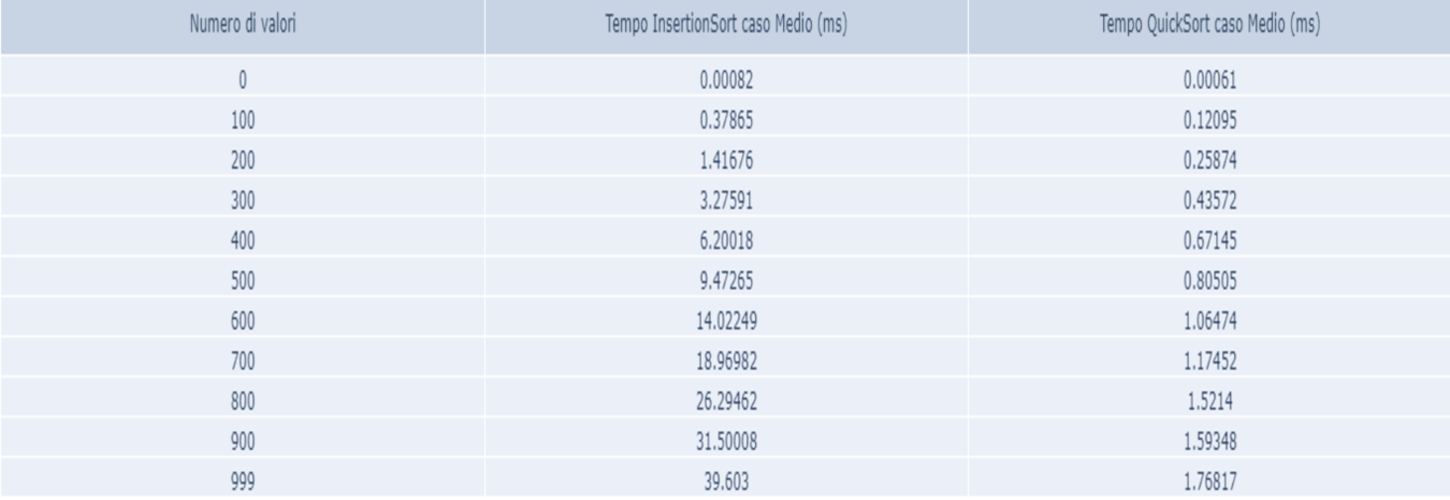
\includegraphics[width=\textwidth]{CasoMedioTabella}
\vspace{-5mm}
\caption{Tabella del caso medio di InsertionSort e QuickSort}
\label{fig:fig1}
\end{figure} \\

\noindent \textit{\bf{Osservazioni:}}
\newline
Si può notare che QuickSort risulta più veloce dell'InsertionSort. \\
In particolare possiamo notare che il blocco, che più aumenta il numero di valori più aumenta il distacco tra i tempi dei due algoritmi, diventando sempre più evidente quanto il quicksort sia migliore dell'insertionsort per una array con valori casuali. \\
\\
Se mettiamo a confronto i due grafici che otteniamo dall'esecuzione di InsertionSort e Quick Sort risulta evidente l'andamento quadratico per l'InsertionSort e come $nlg(n)$ per il QuickSort, infatti otteniamo i seguenti grafici: \\

\begin{figure}[H]
\centering
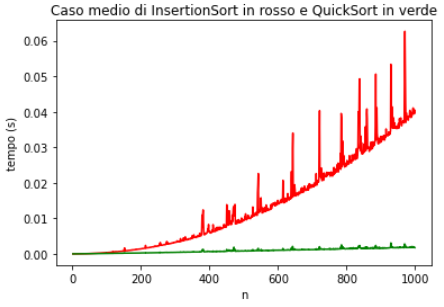
\includegraphics[width=.7\textwidth, height=.6\textheight, keepaspectratio]{CasoMedioGrafico}
\vspace{-5mm}
\caption{Grafico del caso medio di InsertionSort e QuickSort}
\label{fig:fig2}
\end{figure}

% Caso Peggiore InsertionSort e QuickSort
\subsection {Caso Peggiore InsertionSort e QuickSort:}
Per testare invece il caso peggiore di InsertionSort sono stati usati array, sempre di grandezza crescente  da 1 a 1000, ma ordinati in modo decrescente. Infine è stato testato il caso PEGGIORE per QuickSort cioè quando i dati sono ordinati o meglio il caso peggiore di quicksort lo ottengo quando scelgo come pivot l'elemento più grande o più piccolo dell'array, ottenendo così 2 sottoarray con $1$ ed $n-1$ elementi.
Anche in questo caso per avere un risultato più stabile è stata fatta una media su 10 esecuzioni sullo stesso numero di valori. Per costruire la tabella sono stati presi i tempi di esecuzione dopo che il numero di valori dell'array è aumentato di 100 in 100.  \\
\\
\textit{\bf{Risultati InsertionSort e QuickSort caso Peggiore:}} \\
\begin{figure}[h]
\centering
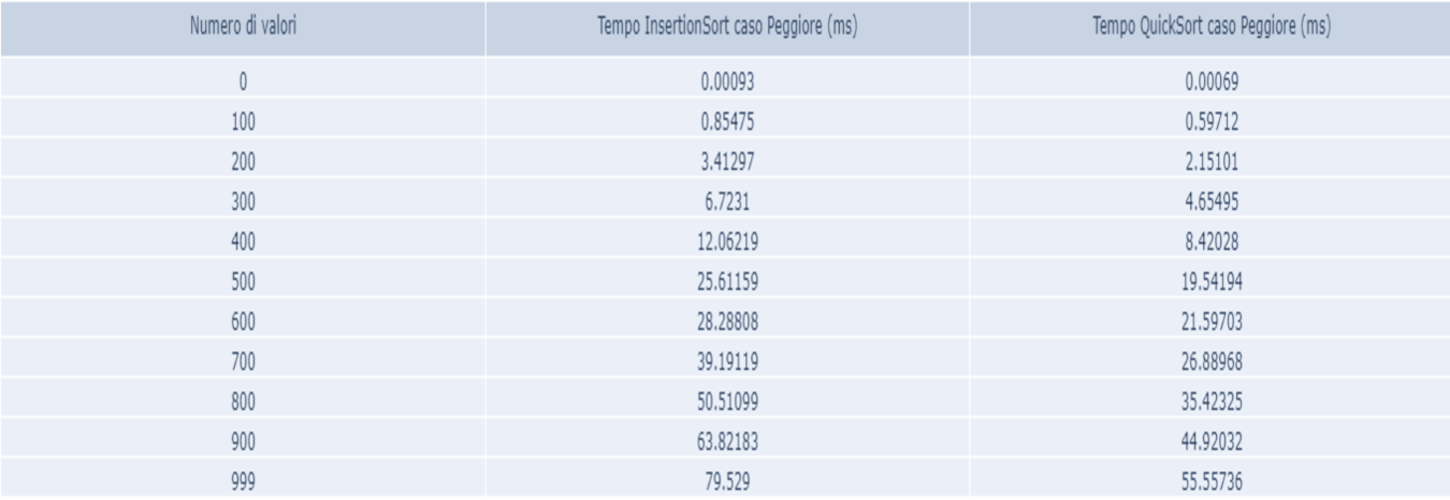
\includegraphics[width=\textwidth]{CasoPeggioreTabella}
\vspace{-5mm}
\caption{Tabella del caso peggiore di Insertionsort e Quicksort}
\label{fig:fig3}
\end{figure} \\


\noindent \textit{\bf{Osservazioni:}}
\newline
\\
Confrontando i grafici dei due algoritmi risulta evidente l'andamento quadratico sia per l'InsertionSort, sia per il QuickSort. DI seguito i due grafici: \\

\begin{figure}[H]
\centering
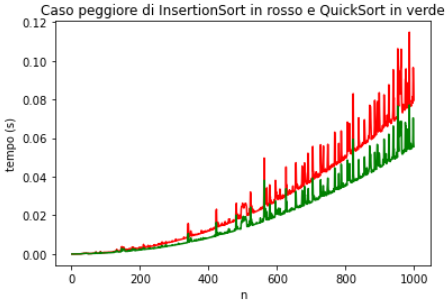
\includegraphics[width=.7\textwidth, height=.6\textheight, keepaspectratio]{CasoPeggioreGrafico}
\vspace{-5mm}
\caption{Grafico del caso peggiore di Insertionsort e Quicksort}
\label{fig:fig4}
\end{figure}



% Caso Migliore InsertionSort
\subsection {Caso Migliore InsertionSort:}
Di seguito viene testato il caso MIGLIORE per InsertionSort cioè quando i dati sono ordinati in ordine crescente. A tal fine è stato utilizzato lo stesso metodo del precedente test, cioè sono stati usati array con numero di elementi crescenti da 1 a 1000 ma sempre ordinati. In questo caso però è stata fatta una media su 15 esecuzioni. Ciò è stato possibile grazie alla velocità di insertionsort nel suo caso migliore, permettendo così di avere un risultato più uniforme. \\
\\
\textit{\bf{Risultati InsertionSort caso Migliore:}} \\
\begin{figure}[h]
\centering
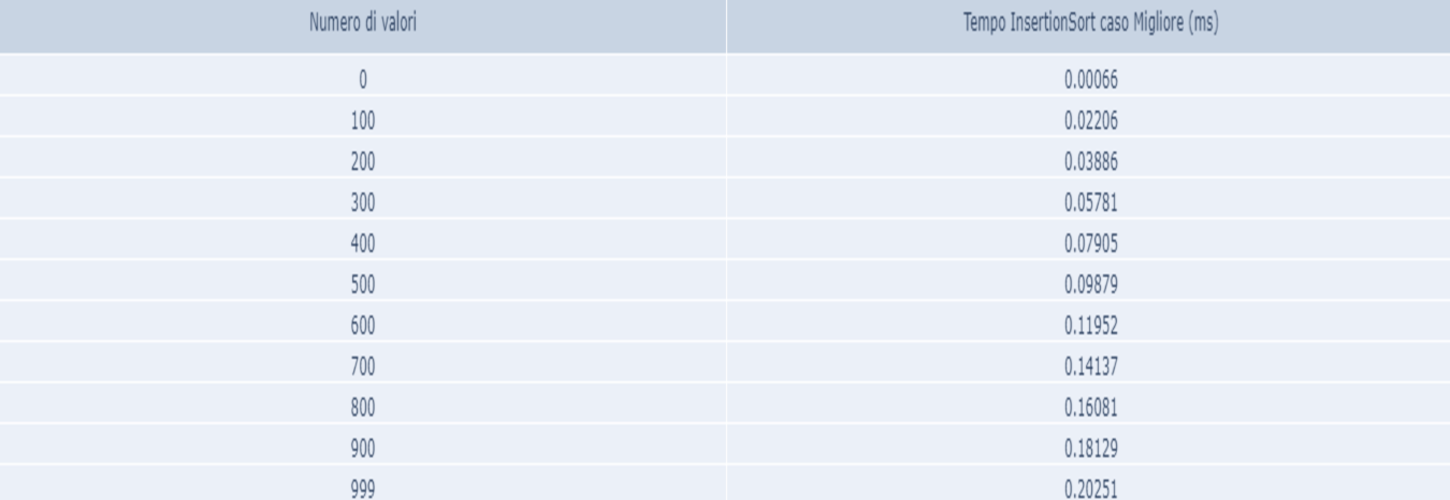
\includegraphics[width=\textwidth]{CasoMiglioreTabella}
\vspace{-5mm}
\caption{Tabella del caso migliore di Insertionsort}
\label{fig:fig5}
\end{figure} \\
\\

\noindent \textit{\bf{Osservazioni:}}
\newline
Notare che InsertionSort risulta molto veloce nel suo caso migliore. É  talmente tanto veloce che riesce ad ordinare l'array più grande in un tempo inferiore rispetto al caso medio di quicksort (0,2 $ms$ di insertionsort contro i 1,7 $ms$ di quicksort). \\
\\
Il grafico che otteniamo dal caso migliore di InsertionSort è il seguente: \\

\begin{figure}[H]
\centering
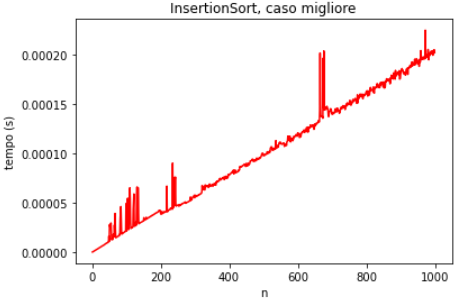
\includegraphics[width=.7\textwidth, height=.6\textheight, keepaspectratio]{CasoMiglioreGrafico}
\vspace{-5mm}
\caption{Grafico del caso migliore di InsertionSort}
\label{fig:fig6}
\end{figure}


% Caso Migliore QuickSort
\subsection {Caso Migliore QuickSort:}
Il caso migliore di quicksort svolgendo ricerche, è risultato che tale situazione accade quando l'array ha dimensioni pari a potenze del 2 e costituisce la sequenza di attraversamento in ordine di un albero binario bilanciato, una serie non facilmente generabile tramite semplici formule. Notando che tale soluzione è risultata discutibile e poco affidabile, motivo per cui, assieme all'effettiva mancanza di un'accurata analisi di questo caso nell'ambito del corso di Algoritmi e Strutture Dati, il caso migliore è stato escluso dalla relazione finale. \\


% Conclusioni
\section {Conclusioni} 
Tranne che nel caso migliore di quicksort, che non è stato possibile implementare correttamente, tutte le performance studiate nella teoria dei diversi casi di insertion sort e quicksort sono state confermate dall'esperimento, indicando come l'analisi matematica degli algoritmi sia effettivamente corretta e visualizzabile anche nella pratica. 

Nello specifico, il caso migliore di insertion sort, ottenuto chiamandolo su array già ordinati, conferma ampiamente l'analisi effettutata matematicamente di un tempo atteso  $\Theta(n)$ in quanto, come osservabile dai risultati ottenuti, i tempi di esecuzione hanno andamento come una funzione lineare.

Similmente viene confermata anche l'ipotesi di costo quadratico $\Theta(n^2)$ nel caso medio (array random) e peggiore (array ordinati al contrario), in cui l'andamento si identifica con una parabola.

Il caso medio di quicksort, invece, implementato chiamandolo su array randomizzati, mostra la correttezza dell'ipotesi di costo $\Theta(n\lg n)$. Confrontandolo con il caso migliore dell'insertion sort per numero di valori alto notiamo che è decisamente inferiore al caso medio del qucik sort.

Infine, in modo simile ai casi medio e peggiore di insertion sort, risulta confermato anche il costo quadratico del caso peggiore di quicksort (array ordinato al contrario o già ordinato), in quanto l'andamento è come una parabola. 

\end{document}